\documentclass[twoside]{book}

% Packages required by doxygen
\usepackage{calc}
\usepackage{doxygen}
\usepackage{graphicx}
\usepackage[utf8]{inputenc}
\usepackage{makeidx}
\usepackage{multicol}
\usepackage{multirow}
\usepackage{textcomp}
\usepackage[table]{xcolor}

% Font selection
\usepackage[T1]{fontenc}
\usepackage{mathptmx}
\usepackage[scaled=.90]{helvet}
\usepackage{courier}
\usepackage{amssymb}
\usepackage{sectsty}
\renewcommand{\familydefault}{\sfdefault}
\allsectionsfont{%
  \fontseries{bc}\selectfont%
  \color{darkgray}%
}
\renewcommand{\DoxyLabelFont}{%
  \fontseries{bc}\selectfont%
  \color{darkgray}%
}

% Page & text layout
\usepackage{geometry}
\geometry{%
  a4paper,%
  top=2.5cm,%
  bottom=2.5cm,%
  left=2.5cm,%
  right=2.5cm%
}
\tolerance=750
\hfuzz=15pt
\hbadness=750
\setlength{\emergencystretch}{15pt}
\setlength{\parindent}{0cm}
\setlength{\parskip}{0.2cm}
\makeatletter
\renewcommand{\paragraph}{%
  \@startsection{paragraph}{4}{0ex}{-1.0ex}{1.0ex}{%
    \normalfont\normalsize\bfseries\SS@parafont%
  }%
}
\renewcommand{\subparagraph}{%
  \@startsection{subparagraph}{5}{0ex}{-1.0ex}{1.0ex}{%
    \normalfont\normalsize\bfseries\SS@subparafont%
  }%
}
\makeatother

% Headers & footers
\usepackage{fancyhdr}
\pagestyle{fancyplain}
\fancyhead[LE]{\fancyplain{}{\bfseries\thepage}}
\fancyhead[CE]{\fancyplain{}{}}
\fancyhead[RE]{\fancyplain{}{\bfseries\leftmark}}
\fancyhead[LO]{\fancyplain{}{\bfseries\rightmark}}
\fancyhead[CO]{\fancyplain{}{}}
\fancyhead[RO]{\fancyplain{}{\bfseries\thepage}}
\fancyfoot[LE]{\fancyplain{}{}}
\fancyfoot[CE]{\fancyplain{}{}}
\fancyfoot[RE]{\fancyplain{}{\bfseries\scriptsize Generated on Thu Apr 2 2015 21\-:27\-:40 for Patient Care System by Doxygen }}
\fancyfoot[LO]{\fancyplain{}{\bfseries\scriptsize Generated on Thu Apr 2 2015 21\-:27\-:40 for Patient Care System by Doxygen }}
\fancyfoot[CO]{\fancyplain{}{}}
\fancyfoot[RO]{\fancyplain{}{}}
\renewcommand{\footrulewidth}{0.4pt}
\renewcommand{\chaptermark}[1]{%
  \markboth{#1}{}%
}
\renewcommand{\sectionmark}[1]{%
  \markright{\thesection\ #1}%
}

% Indices & bibliography
\usepackage{natbib}
\usepackage[titles]{tocloft}
\setcounter{tocdepth}{3}
\setcounter{secnumdepth}{5}
\makeindex

% Hyperlinks (required, but should be loaded last)
\usepackage{ifpdf}
\ifpdf
  \usepackage[pdftex,pagebackref=true]{hyperref}
\else
  \usepackage[ps2pdf,pagebackref=true]{hyperref}
\fi
\hypersetup{%
  colorlinks=true,%
  linkcolor=blue,%
  citecolor=blue,%
  unicode%
}

% Custom commands
\newcommand{\clearemptydoublepage}{%
  \newpage{\pagestyle{empty}\cleardoublepage}%
}


%===== C O N T E N T S =====

\begin{document}

% Titlepage & ToC
\hypersetup{pageanchor=false}
\pagenumbering{roman}
\begin{titlepage}
\vspace*{7cm}
\begin{center}%
{\Large Patient Care System }\\
\vspace*{1cm}
{\large Generated by Doxygen 1.8.6}\\
\vspace*{0.5cm}
{\small Thu Apr 2 2015 21:27:40}\\
\end{center}
\end{titlepage}
\clearemptydoublepage
\tableofcontents
\clearemptydoublepage
\pagenumbering{arabic}
\hypersetup{pageanchor=true}

%--- Begin generated contents ---
\chapter{assets}
\label{md_assets_readme}
\hypertarget{md_assets_readme}{}
As the name implies, it is assets that apply to the web application (i.\-e. css, javascript, and any images used in the web application)

Add notes to this document for added javascript, but I do not see a need to document changes to css or images? 
\chapter{Templates}
\label{md_assets_template_readme}
\hypertarget{md_assets_template_readme}{}
\subsection*{Usage}

For now, use the templates folder as a playground and back up of code. For example, say you are working on ar\-\_\-dashboard and find a layout or functionality that would better suite the doc\-\_\-dashboard. Then, copy the code to a file here for later development.

\subsection*{Naming convetion}

Keep your name on the file. As you can see, I have a file called cb\-\_\-playgound.\-php. I'm using this to get a feel for Bootstrap layout and C\-S\-S.

\subsection*{Also Included}

Of course, this file should keep code that is constantly being reused, see php\-\_\-bootstrap.\-txt for example. This is the bare bones used to create a webpage using php and bootstrap. 
\chapter{control}
\label{md_control_readme}
\hypertarget{md_control_readme}{}
{\bfseries Controller} The controller translates the user's interactions with the view into actions that the model will represent.

Also, responsible for retrieval of information from the database, so look here for the retrieval, and look in {\itshape Model} for formatting retreived data. 

 \subsection*{Control files}

Control file descriptions can be viewed by opening the index.\-html file found in pcs/docs/html folder 
\chapter{Install scripts}
\label{md_db_db_install_scripts_readme}
\hypertarget{md_db_db_install_scripts_readme}{}
\subsection*{Installing the pcs\-\_\-db}

Login to your local mysql from the command line as root user, supply password, then run the \char`\"{}install\-\_\-pcs\-\_\-schema\char`\"{} script. The example below is my linux file path. Your file path will be different.

``` $>$mysql -\/u root -\/p

\begin{quotation}
supply password

\end{quotation}


mysql$>$ . /var/www/pcs/db/db\-\_\-install\-\_\-scripts/install\-\_\-schema\-\_\-v1.0.\-3.\-sql

``` Note\-: The first install should not produce any errors. As Mike edits the database, the install script needs to be updated. So, two options\-:

In the script itself insert a command to delete the old {\bfseries pcs\-\_\-db} and install a fresh new copy.

Or, we'll manually have to delete our local copy and re-\/install.

, just let us know which method to use. , make sure you change the version number of the script....easier to keep track of updates.

\paragraph*{Version Control}

{\bfseries install\-\_\-pcs\-\_\-schema\-\_\-v1.\-0.\-0}\-: \begin{DoxyVerb}* All foreign keys are integer values now.
* Only two user types created:
    - Master  password: masterpass (can access all tables)
    - Login   password: loginpass  (can only read all tables) 
\end{DoxyVerb}


\subsection*{Installing \char`\"{}\-Dummy Data\char`\"{}}

Run the {\itshape dump\-\_\-data.\-sql} script to load up records to the database\-:

``` mysql$>$ . /var/www/pcs/db/db\-\_\-install\-\_\-scripts/dump\-\_\-data.sql

``` Once again, your file path will be different then mine depending on your O\-S and filesystem. 
\chapter{Database Folder}
\label{md_db_readme}
\hypertarget{md_db_readme}{}
\subsection*{Include}


\begin{DoxyEnumerate}
\item Keep copies of the script needed to generate the database in \char`\"{}db\-\_\-install\-\_\-scripts\char`\"{}
\item Keep test scripts in \char`\"{}db\-\_\-test\char`\"{}
\item Keep pics of the E\-R\-D in \char`\"{}db\-\_\-model\char`\"{}
\item Keep a test T\-O\-D\-O list in \char`\"{}db\-\_\-test\char`\"{}
\item Keep the mysql workbench project in \char`\"{}db\-\_\-model\char`\"{}
\end{DoxyEnumerate}

\subsection*{General Note}

See db\-\_\-install\-\_\-scripts to install the pcs\-\_\-db locally

I am by no means a database tester, so if you find a more elegant way to handle testing, go for it. Below is just a suggested method. In any event, we need to document functional queries to the database A\-N\-D have proof that they work. The following is just a suggestion.

\subsection*{Test Scripts}

Test scripts need to include the commands used to access the database. The test script should also include the user type that is used to log in to the database. These test scripts should be direct My\-S\-Q\-L queries, testable in the mysql command prompt. For example\-: a test case needed is to test if the A\-R user can retrieve all appointments (by time and by patient\-I\-D) that have already been made. So, the script should be something similar to the one below\-:

``` // Note\-: This assumes that mysql has been invoked at the command prompt // (i.\-e. shell$>$ mysql) // Also, I am using \$ to represent the command line, and P\-C\-S as the database name.

\$ mysql --host=localhost --user=A\-R --password=arpass P\-C\-S

// Test Case\-: get appointments by time and the patient\-I\-D of the patient // returns a table of the appointments in order of time S\-E\-L\-E\-C\-T Date, Time, Patient\-I\-D F\-R\-O\-M A\-P\-P\-O\-I\-N\-T\-M\-E\-N\-T O\-R\-D\-E\-R B\-Y Date D\-E\-S\-C, Time D\-E\-S\-C

```

\subsubsection*{Saving test results to a file for comparing expected results}

To save the output of a mysql query to a file, simply use the {\itshape I\-N\-T\-O O\-U\-T\-F\-I\-L\-E} command. By default, mysql uses tab separators. We should change this to comma separated (makes it easier to work with in an excel program). Reusing the Query test above, it would look like this\-:

``` S\-E\-L\-E\-C\-T Date, Time, Patient\-I\-D F\-R\-O\-M A\-P\-P\-O\-I\-N\-T\-M\-E\-N\-T O\-R\-D\-E\-R B\-Y Date D\-E\-S\-C, Time D\-E\-S\-C I\-N\-T\-O O\-U\-T\-F\-I\-L\-E '/tmp/test\-\_\-ar\-\_\-appointment\-\_\-retrieve.csv' F\-I\-E\-L\-D\-S T\-E\-R\-M\-I\-N\-A\-T\-E\-D B\-Y ',' E\-N\-C\-L\-O\-S\-E\-D B\-Y '\char`\"{}' L\-I\-N\-E\-S T\-E\-R\-M\-I\-N\-A\-T\-E\-D B\-Y '\par
' ``` W\-A\-R\-N\-I\-N\-G\-: the output file must not exist!!! So, each test case must create a new file. Label each file so it makes sense like above.

As for where to store the file??? It will be different for all of us, cause if you use relative paths it will be different depending on the O\-S being used. So, I would recommend () just storing in a folder called test\-\_\-scripts under {\bfseries T\-H\-I\-S} folder. Then, Paul and I can adjust accordingly.

\subsubsection*{One Master Script}

After each individual test script proves to be working as expected, add it to a \char`\"{}\-Master Test Script\char`\"{}. This script should be able to run all the test cases at once. This way, when we get the database as somewhat expected, we can run the master script after any changes made to the database and the script should point out any errors. 

 \subsection*{Test T\-O\-D\-O}

\subsubsection*{Description}

List individual test cases that need to be tested here.

\subsubsection*{Test Cases}


\begin{DoxyEnumerate}
\item 

 \subsection*{Login to the database\-:}
\end{DoxyEnumerate}

We need 7 users right now to be able to login to the database. Use the following\-:

\begin{TabularC}{2}
\hline
\rowcolor{lightgray}{\bf username }&{\bf password  }\\\cline{1-2}
A\-R &arpass \\\cline{1-2}
E\-M &empass \\\cline{1-2}
Doctor &docpass \\\cline{1-2}
Nurse &nursepass \\\cline{1-2}
M\-R\-S &mrspass \\\cline{1-2}
Master &masterpass \\\cline{1-2}
Login &loginpass \\\cline{1-2}
\end{TabularC}
\subsubsection*{User Priveleges\-: To be completed !!!}

The following list the privileges each user type will need. Note I am using r for read and w for write, and by {\itshape resource} I mean the table(s) in which each user should have access to.


\begin{DoxyEnumerate}
\item Master\-: will have global permissions (much like root) on the database. T\-E\-S\-T\-I\-N\-G P\-U\-R\-P\-O\-S\-E\-S O\-N\-L\-Y (via php and javascript). This user will be removed at deployment
\item Login\-: Login user is used at initial login to check username and password. O\-N\-L\-Y L\-O\-G\-I\-N U\-S\-E\-R S\-H\-O\-U\-L\-D H\-A\-V\-E A\-C\-C\-E\-S\-S T\-O T\-H\-E L\-O\-G\-I\-N T\-A\-B\-L\-E !!!
\end{DoxyEnumerate}

\begin{TabularC}{2}
\hline
\rowcolor{lightgray}{\bf privilege }&{\bf resource  }\\\cline{1-2}
r &L\-O\-G\-I\-N \\\cline{1-2}
r &E\-M\-P\-L\-O\-Y\-E\-E \\\cline{1-2}
\end{TabularC}

\begin{DoxyEnumerate}
\item A\-R
\end{DoxyEnumerate}

\begin{TabularC}{2}
\hline
\rowcolor{lightgray}{\bf privilege }&{\bf resource  }\\\cline{1-2}
wr &A\-P\-P\-O\-I\-N\-T\-M\-E\-N\-T \\\cline{1-2}
wr &P\-A\-T\-I\-E\-N\-T \\\cline{1-2}
wr &A\-D\-D\-R\-E\-S\-S \\\cline{1-2}
r &C\-L\-I\-N\-I\-C \\\cline{1-2}
r &E\-M\-P\-L\-O\-Y\-E\-E \\\cline{1-2}
\end{TabularC}



\begin{DoxyEnumerate}
\item E\-M -\/ Will Need to think about this one B\-U\-T, only read permissions !
\end{DoxyEnumerate}

privilege $\vert$ resource -\/-\/-\/-\/-\/-\/-\/---$\vert$-\/-\/-\/-\/-\/-\/---


\begin{DoxyEnumerate}
\item Doctor
\end{DoxyEnumerate}

\begin{TabularC}{2}
\hline
\rowcolor{lightgray}{\bf privilege }&{\bf resource  }\\\cline{1-2}
rw &A\-P\-P\-O\-I\-N\-T\-M\-E\-N\-T \\\cline{1-2}
rw &M\-E\-D\-I\-C\-A\-T\-I\-O\-N\-S \\\cline{1-2}
rw &T\-E\-A\-T\-E\-M\-E\-N\-T \\\cline{1-2}
rw &M\-E\-D\-\_\-\-R\-E\-C\-O\-R\-D \\\cline{1-2}
rw &A\-L\-L\-E\-R\-G\-Y \\\cline{1-2}
rw &S\-E\-C\-T\-I\-O\-N\-E\-D \\\cline{1-2}
r &P\-A\-T\-I\-E\-N\-T \\\cline{1-2}
r &R\-X \\\cline{1-2}
r &C\-L\-I\-N\-I\-C \\\cline{1-2}
r &E\-M\-P\-L\-O\-Y\-E\-E \\\cline{1-2}
\end{TabularC}



\begin{DoxyEnumerate}
\item Nurse
\end{DoxyEnumerate}

privilege $\vert$ resource -\/-\/-\/-\/-\/-\/-\/---$\vert$-\/-\/-\/-\/-\/-\/---


\begin{DoxyEnumerate}
\item M\-R\-S
\end{DoxyEnumerate}

privilege $\vert$ resource -\/-\/-\/-\/-\/-\/-\/---$\vert$-\/-\/-\/-\/-\/-\/--- 
\chapter{docs}
\label{md_docs_readme}
\hypertarget{md_docs_readme}{}
Contains any relevant docs that we may need to reference during developement. If you find a useful online source, put the link here.

For example, \href{http://www.w3schools.com/bootstrap/}{\tt click\-\_\-me} to go to the bootstrap tutorial provided by w3school.

\subsection*{Adding images}

To add an image to this folder, place the pic in the {\itshape img} folder.



Just look at this readme.\-md in a text editor to see the syntax. Its very straight forward. 
\chapter{Model}
\label{md_model_readme}
\hypertarget{md_model_readme}{}
Contains reusable models.

{\bfseries Model} The model represents data and the rules that govern access to and updates of this data. In enterprise software, a model often serves as a software approximation of a real-\/world process.

Or in plain english, models will be injected into the different user's views. For example, a calendar for the A\-R user is not, in itself, a \char`\"{}view\char`\"{}, it is a model.

When it comes to javascript, we should stick to model generation as\-: (a) create function(s) to create the model, (b) have the model except a {\itshape div} id so the model knows where to put itself.

For php this is not really needed since we can do a direct \char`\"{}include\char`\"{} within the H\-T\-M\-L files. 
\chapter{C\-P\-S\-C4900 Project}
\label{md_readme}
\hypertarget{md_readme}{}
\subsection*{General Notes}

This is the main repository for our school project. Note\-: This description will be deleted in a few weeks.

\subsection*{Markdown}

This is a markdown file. They are very simple to make. We should include one in each folder to give a description of what the folder contains.

For each folder create a file named readme.\-md

``` readme.\-md

This is a literal section. Use these sections to give code examples, terminal command examples, etc ```

\subsection*{Folder structure}

We have a very basic folder structure here with pcs being the root (main) folder. Place the {\itshape pcs} folder in your webserver's host root folder. For Linux, this would be \-\_\-/var/www/pcs.

You will need to configure apache to recognize this folder as being root. If in Linux, go to \-\_\-/etc/apache2\-\_\-. There are two folders named {\itshape sites-\/available} and {\itshape sites-\/enabled}. create a \-\_\-.\-conf\-\_\- file in {\itshape sites-\/available} called {\itshape pcs.\-conf}. Insert the following\-:

``` \section*{P\-C\-S (cpsc4900 project) configuration}

Alias /pcs /var/www/pcs/ $<$Directory \char`\"{}/var/www/pcs/\char`\"{}$>$ Allow\-Override None $<$/\-Directory$>$ ```

Copy this same file into {\itshape sites-\/enabled}

Then, you'll need to restart your server. You can now access the local website with\-:

``` localhost/pcs ```

The first index.\-php page contains a generic greeting to make sure your php and apache server are working properly.

Note\-: Configuration is different for M\-A\-C and Windows, but there should be a httd.\-config file where the above can be accomplished.

\subsection*{P\-H\-P Requirements}


\begin{DoxyEnumerate}
\item For unit testing, see {\itshape tests} folder. You will need to install P\-H\-P\-Unit test Framework.
\item Sessions must be enabled in the php.\-ini file. In Linux, this file is located at\-:

``` /etc/php5/apache2/php.ini ```

You'll need to open the file with root (admin) priveleges...google !

The following need to be set in this folder\-:

``` session.\-save\-\_\-handler = files session.\-save\-\_\-path = \char`\"{}/tmp\char`\"{} session.\-use\-\_\-cookies = 1 ``` Note\-: the save\-\_\-path. You will need to create this folder O\-R use a pre-\/ existing one. I just use the /tmp because cookies are only temporary.

For Unix\-: /tmp is popular For Windows\-: C\-:W\-I\-N\-D\-O\-W\-S\-T\-E\-M\-P is popular

These are the basic settings, I'll make note if/when php.\-ini changes will be required for security. 
\end{DoxyEnumerate}
\chapter{scripts}
\label{md_scripts_readme}
\hypertarget{md_scripts_readme}{}
Folder containing scripts for admin. task.

Examples include\-:


\begin{DoxyEnumerate}
\item Database and Table script backups
\item Automated Test scripts
\item Automated update package scripts.
\end{DoxyEnumerate}

I W\-I\-L\-L T\-R\-Y T\-O S\-T\-I\-C\-K T\-O P\-Y\-T\-H\-O\-N S\-C\-R\-I\-P\-T\-S!!!

Seeing how we are all working on different O\-Ss, I will attempt to keep any needed scripting to python 2.\-7 version. 
\chapter{Tests Folder}
\label{md_tests_readme}
\hypertarget{md_tests_readme}{}
\subsection*{Unit Test}





\subsubsection*{P\-H\-P\-Unit}

Install P\-H\-P\-Unit Test Framework.

Add the php

Refer to \href{https://phpunit.de/manual/current/en/installation.html}{\tt https\-://phpunit.\-de/manual/current/en/installation.\-html} for install and using php unit testing.

For Linux Install, do the following at command line\-:

``` \$\-: wget \href{https://phar.phpunit.de/phpunit.phar}{\tt https\-://phar.\-phpunit.\-de/phpunit.\-phar}

\$\-: chmod +x phpunit.\-phar

\$\-: sudo mv phpunit.\-phar /usr/local/bin/phpunit

\$\-: phpunit --version ```

\paragraph*{Usage}

Create a test class for each unit test. See authenticate\-\_\-test.\-php as an example.

Run test using the following at the command line\-:

``` \$\-: phpunit --bootstrap control/authenticate.\-php tests/authenticate\-\_\-test.\-php ```

To see the test run in verbose\-:

``` \$\-: phpunit --debug --bootstrap control/authenticate.\-php tests/authenticate\-\_\-test.\-php ```

Note\-: the above example assumes that the command prompt is at the \char`\"{}pcs\char`\"{} main folder.

As can be seen in the above command \-\_\---bootstrap--\-\_\- will load the file being tested. This way {\itshape tests/authenticate\-\_\-test.\-php} can access (and test) anything in {\itshape control/authenticate.\-php}

\subsubsection*{T\-O\-D\-O}

Add each command line exection of each unit test into master\-\_\-test\-\_\-script. This script should be able to execute from the command line under the pcs folder and work.

$\ast$$\ast$\-N\-O\-T\-E\-: Keep all file path dependencies relavtive from the pcs root folder. D\-O N\-O\-T U\-S\-E A\-B\-S\-O\-L\-U\-T\-E P\-A\-T\-H\-S $\ast$$\ast$

\subsection*{List of command line running test unit}

The following is a list of command-\/line ran unit test. These eventually need to be put in one script.

``` phpunit --debug --bootstrap control/authenticate.\-php tests/authenticate\-\_\-test.\-php

``` 



\subsubsection*{js\-\_\-unit\-\_\-test}

Under this folder you will find Java\-Script Unit Test (using Q\-Unitsjs).

To run a test\-:


\begin{DoxyEnumerate}
\item Create javascript test file. (This file should be named so the actual file in the system is easy to reference).
\item Add the test js file to {\itshape js\-\_\-test.\-html}
\item Run the test by simple opening the {\itshape js\-\_\-test.\-html} in a browser.
\end{DoxyEnumerate}

That's it !

{\itshape See calendar\-\_\-test.\-js for examples of creating a unit test.} 
\chapter{View}
\label{md_view_readme}
\hypertarget{md_view_readme}{}
\subsection*{Description}

This folder contains the views for different users (i.\-e. the Dashboards, etc). Below is a list of each user type and the files that pertain to them.

Note\-: In some cases the view is redundant (especially with the nurse and doctor). D\-O N\-O\-T R\-E\-P\-E\-A\-T C\-O\-D\-E !!! Section off common view subsections and reuse it.

\subsection*{A\-R Users}

ar\-\_\-dashboard.\-php

\subsection*{E\-M Users}

em\-\_\-dashboard.\-php

\subsection*{Doctor Users}

doc\-\_\-dashboard.\-php

\subsection*{Nurse Users}

nurse\-\_\-dashboard.\-php

\subsection*{M\-R\-S Users}

mrs\-\_\-dashboard.\-php 
\chapter{Hierarchical Index}
\section{Class Hierarchy}
This inheritance list is sorted roughly, but not completely, alphabetically\-:\begin{DoxyCompactList}
\item P\-H\-P\-Unit\-\_\-\-Framework\-\_\-\-Test\-Case\begin{DoxyCompactList}
\item \contentsline{section}{A\-R\-\_\-test\-\_\-suite}{\pageref{classAR__test__suite}}{}
\item \contentsline{section}{Authenticate\-\_\-test}{\pageref{classAuthenticate__test}}{}
\item \contentsline{section}{Authenticate\-\_\-test}{\pageref{classAuthenticate__test}}{}
\end{DoxyCompactList}
\end{DoxyCompactList}

\chapter{Class Index}
\section{Class List}
Here are the classes, structs, unions and interfaces with brief descriptions\-:\begin{DoxyCompactList}
\item\contentsline{section}{\hyperlink{classAR__test__suite}{A\-R\-\_\-test\-\_\-suite} }{\pageref{classAR__test__suite}}{}
\item\contentsline{section}{\hyperlink{classAuthenticate__test}{Authenticate\-\_\-test} }{\pageref{classAuthenticate__test}}{}
\end{DoxyCompactList}

\chapter{File Index}
\section{File List}
Here is a list of all documented files with brief descriptions\-:\begin{DoxyCompactList}
\item\contentsline{section}{control/\hyperlink{authenticate_8php}{authenticate.\-php} }{\pageref{authenticate_8php}}{}
\item\contentsline{section}{control/\hyperlink{db__connect_8php}{db\-\_\-connect.\-php} }{\pageref{db__connect_8php}}{}
\item\contentsline{section}{control/\hyperlink{handle__activity__log_8php}{handle\-\_\-activity\-\_\-log.\-php} }{\pageref{handle__activity__log_8php}}{}
\item\contentsline{section}{control/\hyperlink{handle__apps_8php}{handle\-\_\-apps.\-php} }{\pageref{handle__apps_8php}}{}
\item\contentsline{section}{control/\hyperlink{handle__edit__pat__rec_8php}{handle\-\_\-edit\-\_\-pat\-\_\-rec.\-php} }{\pageref{handle__edit__pat__rec_8php}}{}
\item\contentsline{section}{control/\hyperlink{handle__login_8php}{handle\-\_\-login.\-php} }{\pageref{handle__login_8php}}{}
\item\contentsline{section}{control/\hyperlink{handle__new__allergy_8php}{handle\-\_\-new\-\_\-allergy.\-php} }{\pageref{handle__new__allergy_8php}}{}
\item\contentsline{section}{control/\hyperlink{handle__new__pat__rec_8php}{handle\-\_\-new\-\_\-pat\-\_\-rec.\-php} }{\pageref{handle__new__pat__rec_8php}}{}
\item\contentsline{section}{control/\hyperlink{handle__new__treatment_8php}{handle\-\_\-new\-\_\-treatment.\-php} }{\pageref{handle__new__treatment_8php}}{}
\item\contentsline{section}{control/\hyperlink{logout_8php}{logout.\-php} }{\pageref{logout_8php}}{}
\end{DoxyCompactList}

\chapter{Class Documentation}
\hypertarget{classAR__test__suite}{\section{A\-R\-\_\-test\-\_\-suite Class Reference}
\label{classAR__test__suite}\index{A\-R\-\_\-test\-\_\-suite@{A\-R\-\_\-test\-\_\-suite}}
}
Inheritance diagram for A\-R\-\_\-test\-\_\-suite\-:\begin{figure}[H]
\begin{center}
\leavevmode
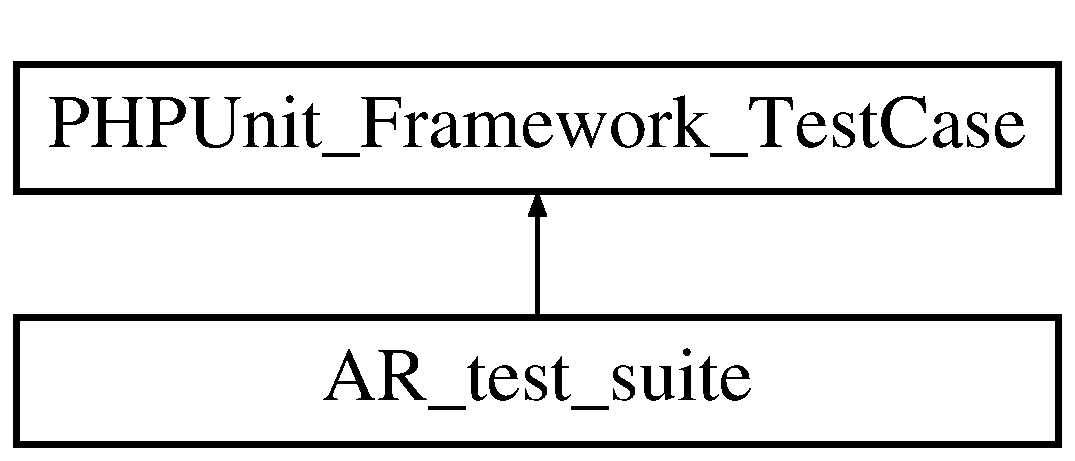
\includegraphics[height=2.000000cm]{classAR__test__suite}
\end{center}
\end{figure}
\subsection*{Public Member Functions}
\begin{DoxyCompactItemize}
\item 
\hypertarget{classAR__test__suite_aa35b707ad07fb6f68e1a5c3f542bd2d9}{{\bfseries test\-\_\-format\-Month} ()}\label{classAR__test__suite_aa35b707ad07fb6f68e1a5c3f542bd2d9}

\item 
\hypertarget{classAR__test__suite_a7767e5f2899f34d98a46841acad7ea0a}{{\bfseries test\-\_\-format\-Day} ()}\label{classAR__test__suite_a7767e5f2899f34d98a46841acad7ea0a}

\item 
\hypertarget{classAR__test__suite_ad086344fb4ee3169f8a146abc641daed}{{\bfseries test\-\_\-format\-Time} ()}\label{classAR__test__suite_ad086344fb4ee3169f8a146abc641daed}

\item 
\hypertarget{classAR__test__suite_a36f2302b55a526e44443f79430d3a71b}{{\bfseries test\-\_\-create\-Date\-Bounds} ()}\label{classAR__test__suite_a36f2302b55a526e44443f79430d3a71b}

\end{DoxyCompactItemize}


\subsection{Detailed Description}
To run\-: \$ phpunit --debug --bootstrap \hyperlink{handle__apps_8php}{control/handle\-\_\-apps.\-php} tests/ar\-\_\-tests.\-php  disabled  disabled 

The documentation for this class was generated from the following file\-:\begin{DoxyCompactItemize}
\item 
tests/ar\-\_\-tests.\-php\end{DoxyCompactItemize}

\hypertarget{classAuthenticate__test}{\section{Authenticate\-\_\-test Class Reference}
\label{classAuthenticate__test}\index{Authenticate\-\_\-test@{Authenticate\-\_\-test}}
}
Inheritance diagram for Authenticate\-\_\-test\-:\begin{figure}[H]
\begin{center}
\leavevmode
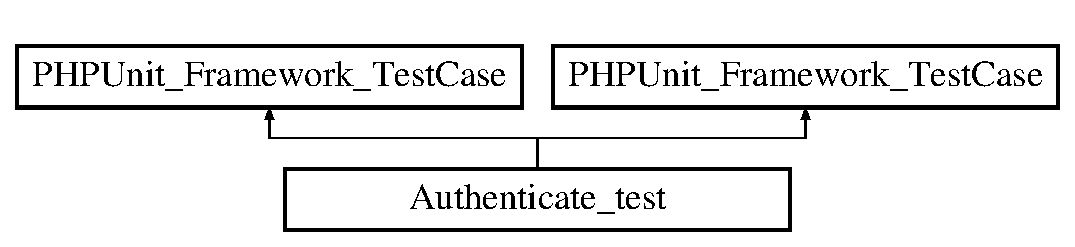
\includegraphics[height=2.000000cm]{classAuthenticate__test}
\end{center}
\end{figure}
\subsection*{Public Member Functions}
\begin{DoxyCompactItemize}
\item 
\hypertarget{classAuthenticate__test_ac55332d4112808f6fea63d5331ab2fde}{{\bfseries test\-Simple\-One\-Word\-Test} ()}\label{classAuthenticate__test_ac55332d4112808f6fea63d5331ab2fde}

\item 
\hypertarget{classAuthenticate__test_aa472c88e650a995f0313bfc174ccffd4}{{\bfseries test\-Empty\-Pass\-Word} ()}\label{classAuthenticate__test_aa472c88e650a995f0313bfc174ccffd4}

\item 
\hyperlink{classAuthenticate__test_a07e33598fb0cc3d9f982d3c76613a7c4}{test\-Dev\-Pass\-Words} ()
\item 
\hypertarget{classAuthenticate__test_ac274cadcd94182c018efb8e0882bf5fe}{{\bfseries test\-Retrieve\-Hashed\-Pwd} ()}\label{classAuthenticate__test_ac274cadcd94182c018efb8e0882bf5fe}

\item 
\hypertarget{classAuthenticate__test_ac7058f883cd0524ba6500251fa481f7e}{{\bfseries test\-Retrieve\-User\-Type} ()}\label{classAuthenticate__test_ac7058f883cd0524ba6500251fa481f7e}

\item 
\hypertarget{classAuthenticate__test_a0b9960005cf588d1aa3a47d716ec9966}{{\bfseries test\-Retrieve\-Employee\-I\-D} ()}\label{classAuthenticate__test_a0b9960005cf588d1aa3a47d716ec9966}

\item 
\hypertarget{classAuthenticate__test_adbb95cf4052bc73408c578c458745ce8}{{\bfseries test\-Date\-Objects} ()}\label{classAuthenticate__test_adbb95cf4052bc73408c578c458745ce8}

\item 
\hypertarget{classAuthenticate__test_adbb95cf4052bc73408c578c458745ce8}{{\bfseries test\-Date\-Objects} ()}\label{classAuthenticate__test_adbb95cf4052bc73408c578c458745ce8}

\end{DoxyCompactItemize}


\subsection{Member Function Documentation}
\hypertarget{classAuthenticate__test_a07e33598fb0cc3d9f982d3c76613a7c4}{\index{Authenticate\-\_\-test@{Authenticate\-\_\-test}!test\-Dev\-Pass\-Words@{test\-Dev\-Pass\-Words}}
\index{test\-Dev\-Pass\-Words@{test\-Dev\-Pass\-Words}!Authenticate_test@{Authenticate\-\_\-test}}
\subsubsection[{test\-Dev\-Pass\-Words}]{\setlength{\rightskip}{0pt plus 5cm}Authenticate\-\_\-test\-::test\-Dev\-Pass\-Words (
\begin{DoxyParamCaption}
{}
\end{DoxyParamCaption}
)}}\label{classAuthenticate__test_a07e33598fb0cc3d9f982d3c76613a7c4}
The Following Passwords are used in Dev\-: \begin{TabularC}{3}
\hline
\rowcolor{lightgray}{\bf username}&{\bf usertype }&{\bf password  }\\\cline{1-3}
mark &A\-R &arpass \\\cline{1-3}
jenny &E\-M &empass \\\cline{1-3}
joe &Doctor &docpass \\\cline{1-3}
alice &Nurse &nursepass \\\cline{1-3}
bob &M\-R\-S &mrspass \\\cline{1-3}
\end{TabularC}


The documentation for this class was generated from the following files\-:\begin{DoxyCompactItemize}
\item 
tests/authenticate\-\_\-test.\-php\item 
tests/cb\-\_\-random\-\_\-test.\-php\end{DoxyCompactItemize}

\chapter{File Documentation}
\hypertarget{authenticate_8php}{\section{control/authenticate.php File Reference}
\label{authenticate_8php}\index{control/authenticate.\-php@{control/authenticate.\-php}}
}
\subsection*{Functions}
\begin{DoxyCompactItemize}
\item 
\hypertarget{authenticate_8php_a290dc9b08db6ef2c2b26400c5b04d750}{{\bfseries init\-\_\-login\-\_\-db\-\_\-conn} ()}\label{authenticate_8php_a290dc9b08db6ef2c2b26400c5b04d750}

\item 
\hyperlink{authenticate_8php_ada393ceabbc91639c41bfb9ffd5e852e}{create\-\_\-hash} (\$string, \$hash\-\_\-method= 'sha256')
\item 
\hyperlink{authenticate_8php_a5654a813bd8d07f822099476c8ebf2aa}{validate\-Login} (\$pass, \$hashed\-\_\-pass, \$hash\-\_\-method= 'sha256')
\item 
\hyperlink{authenticate_8php_a497c371aa0f8c35ba3bcd92befafd960}{retrieve\-Hashed\-Pwd} (\$usr\-\_\-name)
\item 
\hyperlink{authenticate_8php_a9885c0712436d8e44830c054fdc04370}{retrieve\-User\-Type} (\$emp\-\_\-id)
\item 
\hyperlink{authenticate_8php_a40198bd17220f2f39b96138e0b7e5f93}{retrieve\-Employee\-I\-D} (\$usr\-\_\-name)
\item 
\hyperlink{authenticate_8php_a3809efbee136c0e0ec034bcccb98a4a9}{retrieve\-User\-Clinic\-I\-D} (\$emp\-\_\-id)
\end{DoxyCompactItemize}
\subsection*{Variables}
\begin{DoxyCompactItemize}
\item 
\hypertarget{authenticate_8php_a1d006a7b6406a114b344a7e62e438edf}{const {\bfseries U\-N\-I\-Q\-U\-E\-\_\-\-S\-A\-L\-T} '5\&n\-L$\ast$d\-F4'}\label{authenticate_8php_a1d006a7b6406a114b344a7e62e438edf}

\item 
\hypertarget{authenticate_8php_af20afa9ec8b1fdbebf95b48a90e74cab}{{\bfseries \$login\-\_\-conn}}\label{authenticate_8php_af20afa9ec8b1fdbebf95b48a90e74cab}

\end{DoxyCompactItemize}


\subsection{Detailed Description}
Authenticates a user who is attempting to login. Login requires comparing a supplied username and passwords against an entry in the L\-O\-G\-I\-N table. The initial connection to the database is done using a \char`\"{}\-Login\char`\"{} user. This user can only access the Login table. After the username and password have been validated, all following queries are done using the user type of the username.

The functions below support\-: creating a sha-\/256 hash retreiving a hashed password w/ a given username retreiving a \char`\"{}\-User Type\char`\"{} w/ a given Employee\-I\-D validating username and password 

\subsection{Function Documentation}
\hypertarget{authenticate_8php_ada393ceabbc91639c41bfb9ffd5e852e}{\index{authenticate.\-php@{authenticate.\-php}!create\-\_\-hash@{create\-\_\-hash}}
\index{create\-\_\-hash@{create\-\_\-hash}!authenticate.php@{authenticate.\-php}}
\subsubsection[{create\-\_\-hash}]{\setlength{\rightskip}{0pt plus 5cm}create\-\_\-hash (
\begin{DoxyParamCaption}
\item[{}]{\$string, }
\item[{}]{\$hash\-\_\-method = {\ttfamily 'sha256'}}
\end{DoxyParamCaption}
)}}\label{authenticate_8php_ada393ceabbc91639c41bfb9ffd5e852e}
Hashes a string 
\begin{DoxyParams}[1]{Parameters}
string & {\em \$string} & The string to hash \\
\hline
string & {\em \$hash\-\_\-method} & the hash to use \\
\hline
\end{DoxyParams}
\hypertarget{authenticate_8php_a40198bd17220f2f39b96138e0b7e5f93}{\index{authenticate.\-php@{authenticate.\-php}!retrieve\-Employee\-I\-D@{retrieve\-Employee\-I\-D}}
\index{retrieve\-Employee\-I\-D@{retrieve\-Employee\-I\-D}!authenticate.php@{authenticate.\-php}}
\subsubsection[{retrieve\-Employee\-I\-D}]{\setlength{\rightskip}{0pt plus 5cm}retrieve\-Employee\-I\-D (
\begin{DoxyParamCaption}
\item[{}]{\$usr\-\_\-name}
\end{DoxyParamCaption}
)}}\label{authenticate_8php_a40198bd17220f2f39b96138e0b7e5f93}
Retrieves the employee I\-D belonging to the supplied username. 
\begin{DoxyParams}[1]{Parameters}
string & {\em \$usr\-\_\-name} & the login username to find the matching employee id for \\
\hline
\end{DoxyParams}
\begin{DoxyReturn}{Returns}
\mbox{[}int\mbox{]} Returns the employee's I\-D, otherwise returns 0 if a match is not found 
\end{DoxyReturn}
\hypertarget{authenticate_8php_a497c371aa0f8c35ba3bcd92befafd960}{\index{authenticate.\-php@{authenticate.\-php}!retrieve\-Hashed\-Pwd@{retrieve\-Hashed\-Pwd}}
\index{retrieve\-Hashed\-Pwd@{retrieve\-Hashed\-Pwd}!authenticate.php@{authenticate.\-php}}
\subsubsection[{retrieve\-Hashed\-Pwd}]{\setlength{\rightskip}{0pt plus 5cm}retrieve\-Hashed\-Pwd (
\begin{DoxyParamCaption}
\item[{}]{\$usr\-\_\-name}
\end{DoxyParamCaption}
)}}\label{authenticate_8php_a497c371aa0f8c35ba3bcd92befafd960}
Retrieves a hashed password from the Login table. 
\begin{DoxyParams}[1]{Parameters}
string & {\em \$usr\-\_\-name} & The user name of the hashed password that should be retrieved. \\
\hline
\end{DoxyParams}
\begin{DoxyReturn}{Returns}
string the hashed password or 0 if the supplied user name is not in the Login table 
\end{DoxyReturn}
\hypertarget{authenticate_8php_a3809efbee136c0e0ec034bcccb98a4a9}{\index{authenticate.\-php@{authenticate.\-php}!retrieve\-User\-Clinic\-I\-D@{retrieve\-User\-Clinic\-I\-D}}
\index{retrieve\-User\-Clinic\-I\-D@{retrieve\-User\-Clinic\-I\-D}!authenticate.php@{authenticate.\-php}}
\subsubsection[{retrieve\-User\-Clinic\-I\-D}]{\setlength{\rightskip}{0pt plus 5cm}retrieve\-User\-Clinic\-I\-D (
\begin{DoxyParamCaption}
\item[{}]{\$emp\-\_\-id}
\end{DoxyParamCaption}
)}}\label{authenticate_8php_a3809efbee136c0e0ec034bcccb98a4a9}
Retrieves the Clinic I\-D the User belongs to. 
\begin{DoxyParams}{Parameters}
{\em \mbox{[}type\mbox{]}} & \$emp\-\_\-id \mbox{[}description\mbox{]} \\
\hline
\end{DoxyParams}
\begin{DoxyReturn}{Returns}
\mbox{[}type\mbox{]} \mbox{[}description\mbox{]} 
\end{DoxyReturn}
\hypertarget{authenticate_8php_a9885c0712436d8e44830c054fdc04370}{\index{authenticate.\-php@{authenticate.\-php}!retrieve\-User\-Type@{retrieve\-User\-Type}}
\index{retrieve\-User\-Type@{retrieve\-User\-Type}!authenticate.php@{authenticate.\-php}}
\subsubsection[{retrieve\-User\-Type}]{\setlength{\rightskip}{0pt plus 5cm}retrieve\-User\-Type (
\begin{DoxyParamCaption}
\item[{}]{\$emp\-\_\-id}
\end{DoxyParamCaption}
)}}\label{authenticate_8php_a9885c0712436d8e44830c054fdc04370}
Retrieves the \char`\"{}\-User\-Type\char`\"{} field in the E\-M\-P\-L\-O\-Y\-E\-E table. Valid values for \char`\"{}\-User\-Type\char`\"{} are\-: A\-R, E\-M, Doctor, Nurse, or M\-R\-S. 
\begin{DoxyParams}[1]{Parameters}
int & {\em \$emp\-\_\-id} & The id of the employee. \\
\hline
\end{DoxyParams}
\hypertarget{authenticate_8php_a5654a813bd8d07f822099476c8ebf2aa}{\index{authenticate.\-php@{authenticate.\-php}!validate\-Login@{validate\-Login}}
\index{validate\-Login@{validate\-Login}!authenticate.php@{authenticate.\-php}}
\subsubsection[{validate\-Login}]{\setlength{\rightskip}{0pt plus 5cm}validate\-Login (
\begin{DoxyParamCaption}
\item[{}]{\$pass, }
\item[{}]{\$hashed\-\_\-pass, }
\item[{}]{\$hash\-\_\-method = {\ttfamily 'sha256'}}
\end{DoxyParamCaption}
)}}\label{authenticate_8php_a5654a813bd8d07f822099476c8ebf2aa}
Compares a plaintext value to its hash value. Returns non-\/zero if hashes match. 
\begin{DoxyParams}[1]{Parameters}
string & {\em \$pass} & The user submitted password \\
\hline
string & {\em \$hashed\-\_\-pass} & The hashed password pulled from the database \\
\hline
string & {\em \$hash\-\_\-method} & The hashing method used to generate the hashed password \\
\hline
\end{DoxyParams}
\begin{DoxyReturn}{Returns}
Returns true if the supplied password hashed equals the stored hashed password. Otherwise, returns false. 
\end{DoxyReturn}

\hypertarget{db__connect_8php}{\section{control/db\-\_\-connect.php File Reference}
\label{db__connect_8php}\index{control/db\-\_\-connect.\-php@{control/db\-\_\-connect.\-php}}
}
\subsection*{Variables}
\begin{DoxyCompactItemize}
\item 
\hypertarget{db__connect_8php_a6441cca8c9fa11e16d2017e8cb733c10}{{\bfseries \$dsn} = \char`\"{}mysql\-:host=127.\-0.\-0.\-1; dbname=pcs\-\_\-db\char`\"{}}\label{db__connect_8php_a6441cca8c9fa11e16d2017e8cb733c10}

\item 
\hypertarget{db__connect_8php_a0eb82aa5f81cf845de4b36cd653c42cf}{{\bfseries \$username} = \char`\"{}Master\char`\"{}}\label{db__connect_8php_a0eb82aa5f81cf845de4b36cd653c42cf}

\item 
\hypertarget{db__connect_8php_a87911b6664e118fbbfa8da7bb7a04b0f}{{\bfseries \$passwd} = \char`\"{}masterpass\char`\"{}}\label{db__connect_8php_a87911b6664e118fbbfa8da7bb7a04b0f}

\item 
{\bfseries try}
\end{DoxyCompactItemize}


\subsection{Detailed Description}
Handles connecting to the pcs\-\_\-db for getting and setting patient data. A session must be started before this connection is made. After authentication (and the session has started) this connection is reused within global\-\_\-query.\-php 

\subsection{Variable Documentation}
\hypertarget{db__connect_8php_abe4cc9788f52e49485473dc699537388}{\index{db\-\_\-connect.\-php@{db\-\_\-connect.\-php}!try@{try}}
\index{try@{try}!db_connect.php@{db\-\_\-connect.\-php}}
\subsubsection[{try}]{\setlength{\rightskip}{0pt plus 5cm}try}}\label{db__connect_8php_abe4cc9788f52e49485473dc699537388}
{\bfseries Initial value\-:}
\begin{DoxyCode}
\{
    $db\_conn = \textcolor{keyword}{new} PDO($dsn, $username, $passwd)
\end{DoxyCode}

\hypertarget{handle__activity__log_8php}{\section{control/handle\-\_\-activity\-\_\-log.php File Reference}
\label{handle__activity__log_8php}\index{control/handle\-\_\-activity\-\_\-log.\-php@{control/handle\-\_\-activity\-\_\-log.\-php}}
}
\subsection*{Functions}
\begin{DoxyCompactItemize}
\item 
\hyperlink{handle__activity__log_8php_a3bb79b6acd51d8001ecfd557799c83aa}{update\-\_\-activity\-\_\-log} (\$activity\-Type, \$emp\-I\-D, \$rec\-I\-D=0)
\item 
\hypertarget{handle__activity__log_8php_aebdcbbcd60209ede1b77fbbface3fec1}{{\bfseries gen\-\_\-activity\-\_\-pat\-\_\-new\-\_\-rec\-\_\-query} (\$emp\-I\-D, \$prim\-Rec\-I\-D)}\label{handle__activity__log_8php_aebdcbbcd60209ede1b77fbbface3fec1}

\item 
\hypertarget{handle__activity__log_8php_a6699fc94168c0df540182f97ff6dd48e}{{\bfseries gen\-\_\-activity\-\_\-pat\-\_\-edit\-\_\-rec\-\_\-query} (\$emp\-I\-D, \$prim\-Rec\-I\-D)}\label{handle__activity__log_8php_a6699fc94168c0df540182f97ff6dd48e}

\item 
\hypertarget{handle__activity__log_8php_a1c302941777c6678840bc88431474877}{{\bfseries gen\-\_\-activity\-\_\-allergy\-\_\-edit\-\_\-query} (\$emp\-I\-D, \$allergy\-I\-D)}\label{handle__activity__log_8php_a1c302941777c6678840bc88431474877}

\item 
\hypertarget{handle__activity__log_8php_a49b407f45fdbc26675b9534a62a6bb49}{{\bfseries gen\-\_\-activity\-\_\-new\-\_\-allergy\-\_\-query} (\$emp\-I\-D, \$allergy\-I\-D)}\label{handle__activity__log_8php_a49b407f45fdbc26675b9534a62a6bb49}

\item 
\hypertarget{handle__activity__log_8php_a22b8e4fec0508102ba4a76bb9bb1db70}{{\bfseries gen\-\_\-activity\-\_\-user\-\_\-login\-\_\-query} (\$emp\-I\-D)}\label{handle__activity__log_8php_a22b8e4fec0508102ba4a76bb9bb1db70}

\item 
\hypertarget{handle__activity__log_8php_a56b59e5bdad20bd7c2dd26e202c088d5}{{\bfseries gen\-\_\-activity\-\_\-user\-\_\-logout\-\_\-query} (\$emp\-I\-D)}\label{handle__activity__log_8php_a56b59e5bdad20bd7c2dd26e202c088d5}

\item 
\hypertarget{handle__activity__log_8php_a99c26fb9e2ca4c0bc60cf7547e0d9812}{{\bfseries gen\-\_\-activity\-\_\-treat\-\_\-new\-\_\-rec\-\_\-query} (\$emp\-I\-D, \$treat\-I\-D)}\label{handle__activity__log_8php_a99c26fb9e2ca4c0bc60cf7547e0d9812}

\item 
\hypertarget{handle__activity__log_8php_abac3a188ab6499996d203b8252fe0e68}{{\bfseries gen\-\_\-activity\-\_\-treat\-\_\-remove\-\_\-rec\-\_\-query} (\$emp\-I\-D, \$treat\-I\-D)}\label{handle__activity__log_8php_abac3a188ab6499996d203b8252fe0e68}

\end{DoxyCompactItemize}


\subsection{Detailed Description}
Handles updating the A\-C\-T\-I\-V\-I\-T\-Y\-\_\-\-L\-O\-G table. When a user performs an 'activity' worth logging, the table is updated with the I\-D of the user, timestamp, and an id of the record that the user changed, deleted, or created. See the function description for update\-\_\-activity\-\_\-log for activities that get logged. 

\subsection{Function Documentation}
\hypertarget{handle__activity__log_8php_a3bb79b6acd51d8001ecfd557799c83aa}{\index{handle\-\_\-activity\-\_\-log.\-php@{handle\-\_\-activity\-\_\-log.\-php}!update\-\_\-activity\-\_\-log@{update\-\_\-activity\-\_\-log}}
\index{update\-\_\-activity\-\_\-log@{update\-\_\-activity\-\_\-log}!handle_activity_log.php@{handle\-\_\-activity\-\_\-log.\-php}}
\subsubsection[{update\-\_\-activity\-\_\-log}]{\setlength{\rightskip}{0pt plus 5cm}update\-\_\-activity\-\_\-log (
\begin{DoxyParamCaption}
\item[{}]{\$activity\-Type, }
\item[{}]{\$emp\-I\-D, }
\item[{}]{\$rec\-I\-D = {\ttfamily 0}}
\end{DoxyParamCaption}
)}}\label{handle__activity__log_8php_a3bb79b6acd51d8001ecfd557799c83aa}
Updates the activity logs. Activity logs include\-:

Primary\-New Primary\-Edit Allergy\-Edit Allergy\-New User\-Login User\-Logout Treatment\-New Treatment\-Remove 
\begin{DoxyParams}{Parameters}
{\em \mbox{[}string\mbox{]}} & \$activity\-Type See list above \\
\hline
{\em \mbox{[}int\mbox{]}} & \$emp\-I\-D The id of the user who performed the logged activity \\
\hline
{\em \mbox{[}int\mbox{]}} & \$rec\-I\-D If the activity includes updating, creating, or deleting a record, the id of the record must be supplied. For example, Primary\-New activity\-Type would require the primary key (i.\-e. Patient\-I\-D) from the newly created record in the P\-A\-T\-I\-E\-N\-T table \\
\hline
\end{DoxyParams}
\begin{DoxyReturn}{Returns}
\mbox{[}int/string\mbox{]} Returns zero if the activity\-Type is not recognized. Returns 'failed' if the actual query fails to insert the log. Otherwise, returns the last Activity\-\_\-\-L\-O\-G I\-D (i.\-e. the last inserted row's id). 
\end{DoxyReturn}

\hypertarget{handle__apps_8php}{\section{control/handle\-\_\-apps.php File Reference}
\label{handle__apps_8php}\index{control/handle\-\_\-apps.\-php@{control/handle\-\_\-apps.\-php}}
}
\subsection*{Functions}
\begin{DoxyCompactItemize}
\item 
\hyperlink{handle__apps_8php_aa7125df730591e3d6e127d0c82ecf05a}{create\-Date\-Bounds} (\$year, \$month, \$upper\-Bound=false)
\item 
\hyperlink{handle__apps_8php_ae5489b1800879e5690ee1591bcd51989}{get\-\_\-apps\-\_\-per\-\_\-month} (\$year, \$month)
\item 
\hyperlink{handle__apps_8php_a3743147b4aa5a810e2658668b7b738c3}{reformat\-\_\-month\-\_\-apps} (\$app\-\_\-array)
\item 
\hypertarget{handle__apps_8php_af939a69fecfbeb4e55fa0d83f4a4306e}{{\bfseries jsonfy\-\_\-apps\-\_\-per\-\_\-month} (\$app\-\_\-array)}\label{handle__apps_8php_af939a69fecfbeb4e55fa0d83f4a4306e}

\item 
\hyperlink{handle__apps_8php_a64d720df3ce7ec0d8dfcc6bacca5ba0d}{set\-\_\-new\-\_\-app} (\$date\-\_\-time, \$pat\-\_\-id, \$doc\-\_\-id)
\end{DoxyCompactItemize}


\subsection{Detailed Description}
Handles retrieving and setting appointments for the A\-R Dashboard's app\-\_\-form module. See model/app\-\_\-form.\-php for the model details. 

\subsection{Function Documentation}
\hypertarget{handle__apps_8php_aa7125df730591e3d6e127d0c82ecf05a}{\index{handle\-\_\-apps.\-php@{handle\-\_\-apps.\-php}!create\-Date\-Bounds@{create\-Date\-Bounds}}
\index{create\-Date\-Bounds@{create\-Date\-Bounds}!handle_apps.php@{handle\-\_\-apps.\-php}}
\subsubsection[{create\-Date\-Bounds}]{\setlength{\rightskip}{0pt plus 5cm}create\-Date\-Bounds (
\begin{DoxyParamCaption}
\item[{}]{\$year, }
\item[{}]{\$month, }
\item[{}]{\$upper\-Bound = {\ttfamily false}}
\end{DoxyParamCaption}
)}}\label{handle__apps_8php_aa7125df730591e3d6e127d0c82ecf05a}
Helper function\-: Creates either the upper or lower bounds for querying a table that contains a datetime field. Use the \$uppper\-Bound param to determine if the return datetime is upper bound or not. 
\begin{DoxyParams}[1]{Parameters}
integer & {\em \$year} & \\
\hline
integer & {\em \$month} & 0-\/11 \\
\hline
boolean & {\em \$upper\-Bound} & default (false) returns the lower bound of the month. If true, returns the upper bound of the month. For lower bound, the first day of the month with H\-H\-:\-M\-M\-:S\-S = 00\-:00\-:00. For upper bound, uses the last day of the month with H\-H\-:\-M\-M\-:S\-S = 23\-:59\-:59 \\
\hline
\end{DoxyParams}
\begin{DoxyReturn}{Returns}
string returns a datetime format ready for querying a My\-S\-Q\-L datetime column. 
\end{DoxyReturn}
\hypertarget{handle__apps_8php_ae5489b1800879e5690ee1591bcd51989}{\index{handle\-\_\-apps.\-php@{handle\-\_\-apps.\-php}!get\-\_\-apps\-\_\-per\-\_\-month@{get\-\_\-apps\-\_\-per\-\_\-month}}
\index{get\-\_\-apps\-\_\-per\-\_\-month@{get\-\_\-apps\-\_\-per\-\_\-month}!handle_apps.php@{handle\-\_\-apps.\-php}}
\subsubsection[{get\-\_\-apps\-\_\-per\-\_\-month}]{\setlength{\rightskip}{0pt plus 5cm}get\-\_\-apps\-\_\-per\-\_\-month (
\begin{DoxyParamCaption}
\item[{}]{\$year, }
\item[{}]{\$month}
\end{DoxyParamCaption}
)}}\label{handle__apps_8php_ae5489b1800879e5690ee1591bcd51989}
Returns an array of appointments belonging to the month 
\begin{DoxyParams}{Parameters}
{\em \mbox{[}int\mbox{]}} & \$month the month to retrieve appointments for (0-\/11) \\
\hline
\end{DoxyParams}
\begin{DoxyReturn}{Returns}
\mbox{[}tuple array\mbox{]} returns an associative array with a hiearchy of\-:
\end{DoxyReturn}
'Appointment\-I\-D' =$>$ string '2' (length=1) 'App\-Time' =$>$ string '2015-\/03-\/17 11\-:15\-:00' (length=19) 'Showed\-Up' =$>$ string '0' (length=1) 'Clinic\-I\-D' =$>$ string '2' (length=1) 'Patient\-I\-D' =$>$ string '2' (length=1) 'Employee\-I\-D' =$>$ string '1' (length=1) \hypertarget{handle__apps_8php_a3743147b4aa5a810e2658668b7b738c3}{\index{handle\-\_\-apps.\-php@{handle\-\_\-apps.\-php}!reformat\-\_\-month\-\_\-apps@{reformat\-\_\-month\-\_\-apps}}
\index{reformat\-\_\-month\-\_\-apps@{reformat\-\_\-month\-\_\-apps}!handle_apps.php@{handle\-\_\-apps.\-php}}
\subsubsection[{reformat\-\_\-month\-\_\-apps}]{\setlength{\rightskip}{0pt plus 5cm}reformat\-\_\-month\-\_\-apps (
\begin{DoxyParamCaption}
\item[{}]{\$app\-\_\-array}
\end{DoxyParamCaption}
)}}\label{handle__apps_8php_a3743147b4aa5a810e2658668b7b738c3}
Formats the monthly report of appointments into an array of arrays, structured as\-: array('Appointment\-I\-D' =$>$ '2' , \char`\"{}\-App\-Time\char`\"{} =$>$ \char`\"{}2015-\/03-\/17 13\-:00\-:00\char`\"{}, \char`\"{}\-Patient\-I\-D\char`\"{} =$>$ \char`\"{}1\char`\"{}, \char`\"{}\-Employee\-I\-D\char`\"{} =$>$ \char`\"{}2\char`\"{}) 
\begin{DoxyParams}{Parameters}
{\em \mbox{[}type\mbox{]}} & \$app\-\_\-array the array returned by get\-\_\-apps\-\_\-per\-\_\-month \\
\hline
\end{DoxyParams}
\begin{DoxyReturn}{Returns}
\mbox{[}type\mbox{]} \mbox{[}description\mbox{]} 
\end{DoxyReturn}
\hypertarget{handle__apps_8php_a64d720df3ce7ec0d8dfcc6bacca5ba0d}{\index{handle\-\_\-apps.\-php@{handle\-\_\-apps.\-php}!set\-\_\-new\-\_\-app@{set\-\_\-new\-\_\-app}}
\index{set\-\_\-new\-\_\-app@{set\-\_\-new\-\_\-app}!handle_apps.php@{handle\-\_\-apps.\-php}}
\subsubsection[{set\-\_\-new\-\_\-app}]{\setlength{\rightskip}{0pt plus 5cm}set\-\_\-new\-\_\-app (
\begin{DoxyParamCaption}
\item[{}]{\$date\-\_\-time, }
\item[{}]{\$pat\-\_\-id, }
\item[{}]{\$doc\-\_\-id}
\end{DoxyParamCaption}
)}}\label{handle__apps_8php_a64d720df3ce7ec0d8dfcc6bacca5ba0d}
Adds a new appointment to the database. Returns true if the appointment was added. Otherwise, returns false; 
\begin{DoxyParams}{Parameters}
{\em \mbox{[}string\mbox{]}} & \$date\-\_\-time my\-S\-Q\-L formatted datetime string \\
\hline
{\em \mbox{[}int\mbox{]}} & \$pat\-\_\-id the patients id \\
\hline
{\em \mbox{[}int\mbox{]}} & \$doc\-\_\-id the doctors\-\_\-id , user must be logged in for clinic\-\_\-id retrieval. \\
\hline
\end{DoxyParams}

\hypertarget{handle__edit__pat__rec_8php}{\section{control/handle\-\_\-edit\-\_\-pat\-\_\-rec.php File Reference}
\label{handle__edit__pat__rec_8php}\index{control/handle\-\_\-edit\-\_\-pat\-\_\-rec.\-php@{control/handle\-\_\-edit\-\_\-pat\-\_\-rec.\-php}}
}
\subsection*{Variables}
\begin{DoxyCompactItemize}
\item 
if(isset(\$\-\_\-\-P\-O\-S\-T\mbox{[}'criteria'\mbox{]})\&\&isset(\$\-\_\-\-P\-O\-S\-T\mbox{[}'value'\mbox{]})) \\*
else if(isset(\$\-\_\-\-P\-O\-S\-T\mbox{[}'patid'\mbox{]})\&\&isset(\$\-\_\-\-P\-O\-S\-T\mbox{[}'fname'\mbox{]})\&\&isset(\$\-\_\-\-P\-O\-S\-T\mbox{[}'lname'\mbox{]})\&\&isset(\$\-\_\-\-P\-O\-S\-T\mbox{[}'ssn'\mbox{]})\&\&isset(\$\-\_\-\-P\-O\-S\-T\mbox{[}'bday'\mbox{]})\&\&isset(\$\-\_\-\-P\-O\-S\-T\mbox{[}'phone\-Num'\mbox{]})\&\&isset(\$\-\_\-\-P\-O\-S\-T\mbox{[}'gender'\mbox{]})\&\&isset(\$\-\_\-\-P\-O\-S\-T\mbox{[}'street'\mbox{]})\&\&isset(\$\-\_\-\-P\-O\-S\-T\mbox{[}'city'\mbox{]})\&\&isset(\$\-\_\-\-P\-O\-S\-T\mbox{[}'state'\mbox{]})\&\&isset(\$\-\_\-\-P\-O\-S\-T\mbox{[}'zip'\mbox{]})) {\bfseries else}
\end{DoxyCompactItemize}


\subsection{Detailed Description}
Handles all A\-J\-A\-X requests from the edit\-\_\-pat\-\_\-record\-\_\-model.\-php. See control/handle\-\_\-edit\-\_\-pat\-\_\-prim\-\_\-rec.\-js for A\-J\-A\-X requests

This file handles; (a) request for returning patient primary records based on search criteria (S\-S\-N, Lname, or Patient\-Id), (b) request for updating a patient's primary record. 

\subsection{Variable Documentation}
\hypertarget{handle__edit__pat__rec_8php_ae977646182091e9d676fab7abaa34912}{\index{handle\-\_\-edit\-\_\-pat\-\_\-rec.\-php@{handle\-\_\-edit\-\_\-pat\-\_\-rec.\-php}!else@{else}}
\index{else@{else}!handle_edit_pat_rec.php@{handle\-\_\-edit\-\_\-pat\-\_\-rec.\-php}}
\subsubsection[{else}]{\setlength{\rightskip}{0pt plus 5cm}if (isset(\$\-\_\-\-P\-O\-S\-T\mbox{[}'criteria'\mbox{]})\&\&isset(\$\-\_\-\-P\-O\-S\-T\mbox{[}'value'\mbox{]})) else if (isset(\$\-\_\-\-P\-O\-S\-T\mbox{[}'patid'\mbox{]})\&\&isset(\$\-\_\-\-P\-O\-S\-T\mbox{[}'fname'\mbox{]})\&\&isset(\$\-\_\-\-P\-O\-S\-T\mbox{[}'lname'\mbox{]})\&\&isset(\$\-\_\-\-P\-O\-S\-T\mbox{[}'ssn'\mbox{]})\&\&isset(\$\-\_\-\-P\-O\-S\-T\mbox{[}'bday'\mbox{]})\&\&isset(\$\-\_\-\-P\-O\-S\-T\mbox{[}'phone\-Num'\mbox{]})\&\&isset(\$\-\_\-\-P\-O\-S\-T\mbox{[}'gender'\mbox{]})\&\&isset(\$\-\_\-\-P\-O\-S\-T\mbox{[}'street'\mbox{]})\&\&isset(\$\-\_\-\-P\-O\-S\-T\mbox{[}'city'\mbox{]})\&\&isset(\$\-\_\-\-P\-O\-S\-T\mbox{[}'state'\mbox{]})\&\&isset(\$\-\_\-\-P\-O\-S\-T\mbox{[}'zip'\mbox{]})) else}}\label{handle__edit__pat__rec_8php_ae977646182091e9d676fab7abaa34912}
{\bfseries Initial value\-:}
\begin{DoxyCode}
\{
    header(\textcolor{stringliteral}{"Location: ../PermissionDenied.php"})
\end{DoxyCode}

\hypertarget{handle__login_8php}{\section{control/handle\-\_\-login.php File Reference}
\label{handle__login_8php}\index{control/handle\-\_\-login.\-php@{control/handle\-\_\-login.\-php}}
}
\subsection*{Variables}
\begin{DoxyCompactItemize}
\item 
if(\$is\-\_\-dev) if(isset(\$\-\_\-\-P\-O\-S\-T\mbox{[}'user\-Name'\mbox{]})\&\&!empty(\$\-\_\-\-P\-O\-S\-T\mbox{[}'user\-Name'\mbox{]})\&\&!empty(\$\-\_\-\-P\-O\-S\-T\mbox{[}'pass\-Word'\mbox{]})\&\&isset(\$\-\_\-\-P\-O\-S\-T\mbox{[}'user\-Name'\mbox{]})) \hyperlink{handle__login_8php_a8ccfa260cf1b11e9f57f551d5e02f56e}{else}
\end{DoxyCompactItemize}


\subsection{Detailed Description}
Handles initial logging in. This file excepts a username and password, checks for valigation using \hyperlink{authenticate_8php}{control/authenticate.\-php}, and redirects the user upon authentication to the correct user Dashboard. This is where the Session starts. Session data includes\-: (a)Employee\-I\-D, (b) User\-Type, (c) Clinic\-I\-D, (d) and a timestamp, for logging when a user has logged in. This session data is persistant until a user logs out O\-R the session expires due to no activity (currently set to 10 minutes). 

\subsection{Variable Documentation}
\hypertarget{handle__login_8php_a8ccfa260cf1b11e9f57f551d5e02f56e}{\index{handle\-\_\-login.\-php@{handle\-\_\-login.\-php}!else@{else}}
\index{else@{else}!handle_login.php@{handle\-\_\-login.\-php}}
\subsubsection[{else}]{\setlength{\rightskip}{0pt plus 5cm}if (\$is\-\_\-dev) if (isset(\$\-\_\-\-P\-O\-S\-T\mbox{[}'user\-Name'\mbox{]})\&\&!empty(\$\-\_\-\-P\-O\-S\-T\mbox{[}'user\-Name'\mbox{]})\&\&!empty(\$\-\_\-\-P\-O\-S\-T\mbox{[}'pass\-Word'\mbox{]})\&\&isset(\$\-\_\-\-P\-O\-S\-T\mbox{[}'user\-Name'\mbox{]})) else}}\label{handle__login_8php_a8ccfa260cf1b11e9f57f551d5e02f56e}
{\bfseries Initial value\-:}
\begin{DoxyCode}
\{                                          
  header(\textcolor{stringliteral}{"Location: ../index.php"})
\end{DoxyCode}
username$\vert$ usertype $\vert$ password -\/-\/-\/-\/-\/-\/-\/-\/-\/-\/-\/-\/-\/-\/-\/-\/-\/-\/---$\vert$-\/-\/-\/-\/-\/-\/--- mark $\vert$ A\-R $\vert$ arpass jenny $\vert$ E\-M $\vert$ empass joe $\vert$ Doctor $\vert$ docpass alice $\vert$ Nurse $\vert$ nursepass bob $\vert$ M\-R\-S $\vert$ mrspass

Database Access username $\vert$ password -\/-\/-\/-\/-\/-\/---$\vert$-\/-\/-\/-\/-\/-\/-\/--- Login logpass Master $\vert$ Master 
\hypertarget{handle__new__allergy_8php}{\section{control/handle\-\_\-new\-\_\-allergy.php File Reference}
\label{handle__new__allergy_8php}\index{control/handle\-\_\-new\-\_\-allergy.\-php@{control/handle\-\_\-new\-\_\-allergy.\-php}}
}
\subsection*{Variables}
\begin{DoxyCompactItemize}
\item 
if(isset(\$\-\_\-\-P\-O\-S\-T\mbox{[}'allergy\-Name'\mbox{]})\&\&isset(\$\-\_\-\-P\-O\-S\-T\mbox{[}'severity'\mbox{]})\&\&isset(\$\-\_\-\-P\-O\-S\-T\mbox{[}'patid'\mbox{]})) {\bfseries else}
\end{DoxyCompactItemize}


\subsection{Detailed Description}
Handles A\-J\-A\-X request related to creating new allergy records. See control/handle\-\_\-new\-\_\-allergy.\-js for A\-J\-A\-X requests 

\subsection{Variable Documentation}
\hypertarget{handle__new__allergy_8php_a53ff9376e169336e69c1f774c451060b}{\index{handle\-\_\-new\-\_\-allergy.\-php@{handle\-\_\-new\-\_\-allergy.\-php}!else@{else}}
\index{else@{else}!handle_new_allergy.php@{handle\-\_\-new\-\_\-allergy.\-php}}
\subsubsection[{else}]{\setlength{\rightskip}{0pt plus 5cm}if (isset(\$\-\_\-\-P\-O\-S\-T\mbox{[}'allergy\-Name'\mbox{]})\&\&isset(\$\-\_\-\-P\-O\-S\-T\mbox{[}'severity'\mbox{]})\&\&isset(\$\-\_\-\-P\-O\-S\-T\mbox{[}'patid'\mbox{]})) else}}\label{handle__new__allergy_8php_a53ff9376e169336e69c1f774c451060b}
{\bfseries Initial value\-:}
\begin{DoxyCode}
\{
    echo \textcolor{stringliteral}{"failed"}
\end{DoxyCode}

\hypertarget{handle__new__pat__rec_8php}{\section{control/handle\-\_\-new\-\_\-pat\-\_\-rec.php File Reference}
\label{handle__new__pat__rec_8php}\index{control/handle\-\_\-new\-\_\-pat\-\_\-rec.\-php@{control/handle\-\_\-new\-\_\-pat\-\_\-rec.\-php}}
}
\subsection*{Variables}
\begin{DoxyCompactItemize}
\item 
if(isset(\$\-\_\-\-P\-O\-S\-T\mbox{[}'first\-Name'\mbox{]})\&\&isset(\$\-\_\-\-P\-O\-S\-T\mbox{[}'last\-Name'\mbox{]})\&\&isset(\$\-\_\-\-P\-O\-S\-T\mbox{[}'pat\-S\-S\-N'\mbox{]})\&\&isset(\$\-\_\-\-P\-O\-S\-T\mbox{[}'phone\-Num'\mbox{]})\&\&isset(\$\-\_\-\-P\-O\-S\-T\mbox{[}'gender\-Chk'\mbox{]})\&\&isset(\$\-\_\-\-P\-O\-S\-T\mbox{[}'pat\-Bday'\mbox{]})\&\&isset(\$\-\_\-\-P\-O\-S\-T\mbox{[}'pat\-St\-Add'\mbox{]})\&\&isset(\$\-\_\-\-P\-O\-S\-T\mbox{[}'pat\-City'\mbox{]})\&\&isset(\$\-\_\-\-P\-O\-S\-T\mbox{[}'pat\-Zip'\mbox{]})\&\&isset(\$\-\_\-\-P\-O\-S\-T\mbox{[}'pat\-State'\mbox{]})) {\bfseries else}
\end{DoxyCompactItemize}


\subsection{Detailed Description}
Handles A\-J\-A\-X requests for creating new patient primary records. See handle\-\_\-new\-\_\-pat\-\_\-prim\-\_\-rec.\-js for A\-J\-A\-X requests 

\subsection{Variable Documentation}
\hypertarget{handle__new__pat__rec_8php_a368238c368fe2cdb1f7ddccb3d054563}{\index{handle\-\_\-new\-\_\-pat\-\_\-rec.\-php@{handle\-\_\-new\-\_\-pat\-\_\-rec.\-php}!else@{else}}
\index{else@{else}!handle_new_pat_rec.php@{handle\-\_\-new\-\_\-pat\-\_\-rec.\-php}}
\subsubsection[{else}]{\setlength{\rightskip}{0pt plus 5cm}if (isset(\$\-\_\-\-P\-O\-S\-T\mbox{[}'first\-Name'\mbox{]})\&\&isset(\$\-\_\-\-P\-O\-S\-T\mbox{[}'last\-Name'\mbox{]})\&\&isset(\$\-\_\-\-P\-O\-S\-T\mbox{[}'pat\-S\-S\-N'\mbox{]})\&\&isset(\$\-\_\-\-P\-O\-S\-T\mbox{[}'phone\-Num'\mbox{]})\&\&isset(\$\-\_\-\-P\-O\-S\-T\mbox{[}'gender\-Chk'\mbox{]})\&\&isset(\$\-\_\-\-P\-O\-S\-T\mbox{[}'pat\-Bday'\mbox{]})\&\&isset(\$\-\_\-\-P\-O\-S\-T\mbox{[}'pat\-St\-Add'\mbox{]})\&\&isset(\$\-\_\-\-P\-O\-S\-T\mbox{[}'pat\-City'\mbox{]})\&\&isset(\$\-\_\-\-P\-O\-S\-T\mbox{[}'pat\-Zip'\mbox{]})\&\&isset(\$\-\_\-\-P\-O\-S\-T\mbox{[}'pat\-State'\mbox{]})) else}}\label{handle__new__pat__rec_8php_a368238c368fe2cdb1f7ddccb3d054563}
{\bfseries Initial value\-:}
\begin{DoxyCode}
\{
    header(\textcolor{stringliteral}{"Location: ../PermissionDenied.php"})
\end{DoxyCode}

\hypertarget{handle__new__treatment_8php}{\section{control/handle\-\_\-new\-\_\-treatment.php File Reference}
\label{handle__new__treatment_8php}\index{control/handle\-\_\-new\-\_\-treatment.\-php@{control/handle\-\_\-new\-\_\-treatment.\-php}}
}
\subsection*{Variables}
\begin{DoxyCompactItemize}
\item 
if(isset(\$\-\_\-\-P\-O\-S\-T\mbox{[}'get\-Doc\-List'\mbox{]})\&\&(\$\-\_\-\-P\-O\-S\-T\mbox{[}'get\-Doc\-List'\mbox{]}==\char`\"{}true\char`\"{})) \\*
else if(isset(\$\-\_\-\-P\-O\-S\-T\mbox{[}'diagnosis'\mbox{]})\&\&isset(\$\-\_\-\-P\-O\-S\-T\mbox{[}'descript'\mbox{]})) {\bfseries else}
\end{DoxyCompactItemize}


\subsection{Detailed Description}
Handles A\-J\-A\-X requests for creating treatment records. Also handles returning a list of doctors for treatments that include doctor referrals.

See control/handle\-\_\-new\-\_\-treatment.\-js for A\-J\-A\-X requests 

\subsection{Variable Documentation}
\hypertarget{handle__new__treatment_8php_af193675f4a9a0a5b39ba0fdfe4ead91d}{\index{handle\-\_\-new\-\_\-treatment.\-php@{handle\-\_\-new\-\_\-treatment.\-php}!else@{else}}
\index{else@{else}!handle_new_treatment.php@{handle\-\_\-new\-\_\-treatment.\-php}}
\subsubsection[{else}]{\setlength{\rightskip}{0pt plus 5cm}if (isset(\$\-\_\-\-P\-O\-S\-T\mbox{[}'get\-Doc\-List'\mbox{]})\&\&(\$\-\_\-\-P\-O\-S\-T\mbox{[}'get\-Doc\-List'\mbox{]}==\char`\"{}true\char`\"{})) else if (isset(\$\-\_\-\-P\-O\-S\-T\mbox{[}'diagnosis'\mbox{]})\&\&isset(\$\-\_\-\-P\-O\-S\-T\mbox{[}'descript'\mbox{]})) else}}\label{handle__new__treatment_8php_af193675f4a9a0a5b39ba0fdfe4ead91d}
{\bfseries Initial value\-:}
\begin{DoxyCode}
\{
    echo \textcolor{stringliteral}{"err:14"}
\end{DoxyCode}

\hypertarget{logout_8php}{\section{control/logout.php File Reference}
\label{logout_8php}\index{control/logout.\-php@{control/logout.\-php}}
}


\subsection{Detailed Description}
Handles a user logging out. During logout, the session is stopped and an activity log is added to the A\-C\-T\-I\-V\-I\-T\-Y\-\_\-\-L\-O\-G 
%--- End generated contents ---

% Index
\newpage
\phantomsection
\addcontentsline{toc}{chapter}{Index}
\printindex

\end{document}
